\section{Theorie}
\label{sec:Theorie}

Im Allgemeinen können Kräfte, die auf einen Körper einwirken, dessen Form und Volumen beeinflussen. 
Eine pro Fläche wirkende Kraft wird dabei als Spannung bezeichnet, wobei die Normalspannung $\sigma$, die auch als Druck bezeichnet wird,
diejenige Kraft pro Fläche ist, die senkrecht zur Oberfläche des Körpers auf diesen einwirkt. Für eine eindimensionale Änderung der
Körperform gilt dabei der Zusammenhang \begin{equation}
    \sigma = E \frac{\Delta L}L \text{,}
\end{equation}

 der das Hookesche Gesetz beschreibt. Dabei ist $L$ die Dimension des Körpers ohne Krafteinwirkung und $\Delta L$ die eindimensionale
Verformung, die durch die wirkende Kraft zustande kommt. Der Faktor $E$ gibt den Elastizitätsmodul an.

Die Bestimmung eines Elastizitätsmoduls erfolgt in dieser Versuchsreihe über eine Biegung des zu 
untersuchenden Materials. 

\subsection{Einseitige Einspannung}

\begin{figure}
    \centering
    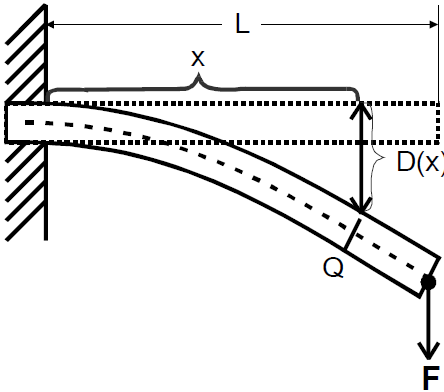
\includegraphics[height=6cm]{data/bild_1}
    \caption{Einseitige Einspannung}
\end{figure}

Die gestrichelte Linie zeigt die sogenannte neutrale Faser, die sich bei der Biegung nicht in der Länge verändert. 
Über dieser kommt es zur Streckung, und darunter zur Stauchung des Materials. Am Querschnitt $Q$ greifen damit Zug- und Druckspannungen
an, die bei gleichem Betrag entgegengesetzt wirken, wodurch ein Drehmoment $M_{\sigma}$ entsteht. Dieses lässt sich durch \begin{equation}
    M_{\sigma} = \int_Q y\sigma(y)\text{d}q
\end{equation}

darstellen, wobei $y$ der Abstand von $\text{d}q$ zur neutralen Faser ist.

Bei konstanter Kraft gleicht sich das durch sie wirkende Drehmoment $M_F$ mit dem eben beschrieben Drehmoment aus. Daraus folgt \begin{equation}
    \label{eqn:m_gleich}
    \int_Q y\sigma(y)\text{d}q = F (L - x) 
\end{equation}

Mit \begin{equation}
    \sigma (y) = E y \frac{\text{d}^2 D}{\text{d} x^2}
\end{equation}

lässt sich dann durch Integration über $Q$ von Gleichung \eqref{eqn:m_gleich} die $x$- abhängige Auslenkung bestimmen:
\begin{equation}
    D(x) = \frac{F}{2EI} \Bigl( L x^2 - \frac{x^3}3 \Bigr)
    \label{eqn:D1_gleich}
\end{equation}
Diese Gleichung gilt nur unter einer Kleinwinkelnäherung, also  für große $R$. Da die Durchbiegung 
in dem Fall eine geringe Kurvenkrümmung erzeugt, kann diese Näherung angenommen werden.

Dabei ist $I$ das Flächenträgheitsmoment \begin{equation}
    I := \int_Q y^2 \text{d}q
    \label{eqn:I}
\end{equation}

Damit ist der Elastizitätsmodul nur durch $x$ und die davon abhängige Durchbiegung $D$ zu bestimmen.

\subsection{Beidseitige Auflage}
\begin{figure}
    \centering
    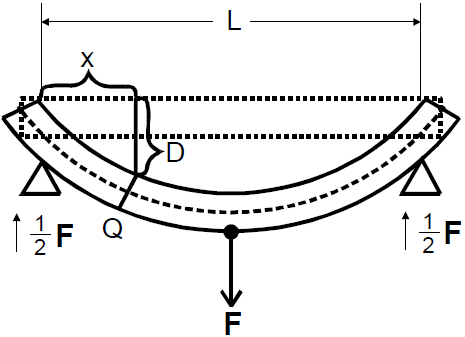
\includegraphics[height=5cm]{data/bild_2}
    \caption{Beidseitige Auflage}
    \label{fig:2th}
\end{figure}

\FloatBarrier

Da hier der Stab beidseitig aufliegt und eine Auslenkung mit einem Gewicht in der Mitte der beiden Auflagepunkte gemessen wird, ist hierbei
vom voherigen Aufbau abweichend das Drehmoment \begin{align}
M_F &= - \frac{F}2 x       &   0 \leq x \leq L/2 \\
M_F &= - \frac{F}2 (L - x) & L/2 \leq x \leq L
\end{align}

Dadurch kommt die Funktion für die $x$- abhängige Auslenkung folgendermaßen zustande: \begin{equation}
   D(x) = \frac{F}{48EI} \bigl( 3L^2 x -4x^3 \bigr)
   \label{eqn:D2_gleich}
\end{equation} für $0 \leq x \leq L/2$

und für $L/2 \leq x \leq L$ gilt entsprechend \begin{equation}
    D(x) = \frac{F}{48EI} \bigl( 4x^3 - 12Lx^2 + 9L^2 x - L^3 \bigr)
    \label{eqn:D3_gleich}
\end{equation}

